% --- ETUDE DE CAS ---
\newpage

\section*{AAV}
\addcontentsline{toc}{section}{AAV}
\begin{itemize}
	\item [5] Appliquer les règles de création des composants
	\item [6] Construire et manipuler des données en JSON
	\item [2] Reconnaître les cycles de vie d'un composant
	\item [3] Réaliser la modélisation d'une application Frontend
	\item [5] Utiliser un framework Frontend
	\item [5] Utiliser l’une des librairies de style (Bootstrap, Tailwind, etc.)
\end{itemize}

\newpage

\section*{Étude de cas~: Front-end}
\addcontentsline{toc}{section}{Étude de cas~: Front-end}

\subsection*{Mots clés}
\phantomsection
\addcontentsline{toc}{subsection}{Mots clés}
\begin{itemize}
	\item Json
	\item Composant
	\item React
	\item Front-end
	\item Wireframe
	\item Redux
	\item Tailwind CSS
	\item useEffect
	\item Axios
	\item DOM
\end{itemize}

\subsection*{Contexte}
\phantomsection
\addcontentsline{toc}{subsection}{Contexte}
\noindent Yanis développe le front-end d'une application avec des composants modulaires via React et Tailwind CSS. Il rencontre des erreurs d'initialisation car les données JSON requises par son composant ne sont pas complètement chargées au moment du rendu de la page.

\subsection*{Problématique}
\phantomsection
\addcontentsline{toc}{subsection}{Problématique}
\noindent Comment gérer efficacement le cycle de vie des composants et le chargement asynchrone des données dans une application React pour éviter les erreurs d'affichage ?

\subsection*{Contraintes}
\phantomsection
\addcontentsline{toc}{subsection}{Contraintes}
\begin{itemize}
	\item React
	\item Tailwind CSS
	\item JSON
\end{itemize}

\subsection*{Généralisation}
\phantomsection
\addcontentsline{toc}{subsection}{Généralisation}
\begin{itemize}
	\item Front-end
	\item Composant
\end{itemize}

\subsection*{Livrables}
\phantomsection
\addcontentsline{toc}{subsection}{Livrables}
\begin{itemize}
	\item Diagramme séquence
	\item Code source de l'application Front-end
\end{itemize}

\newpage

\subsection*{Pistes de solutions}
\phantomsection
\addcontentsline{toc}{subsection}{Pistes de solutions}
\begin{itemize}
	\item Se renseigner sur le cycle de vie des composants React et les hooks useEffect
	\item Se renseigner sur Redux
	\item Concevoir des composants indépendants et réutilisables
\end{itemize}

\subsection*{Plan d'actions}
\phantomsection
\addcontentsline{toc}{subsection}{Plan d'actions}
\begin{itemize}
	\item DMC
	\item ER
	\item Étudier le fonctionnement de React (composants, hooks, états)
	\item Voir l'architecture de l'application via des wireframes.
	\item Initialiser un projet React/Next.js.
	\item Créer les premiers composants
	\item Installer et configurer Axios 
	\item Implémenter les hooks (useState, useEffect) pour gérer correctement les données et le cycle de vie des composants.
	\item Gérer la navigation et le routage entre les différentes pages de l'appli
\end{itemize}

\newpage

\section*{Définition~: Mots clés}
\phantomsection
\addcontentsline{toc}{section}{Définition~: Mots clés}

\subsubsection*{JSON}
\phantomsection
\addcontentsline{toc}{subsection}{JSON}

\noindent \textbf{JSON} (\textit{JavaScript Object Notation}) est un \textbf{format d'échange de données} léger, textuel et lisible par l'humain, devenu le standard de la communication entre un front-end et une API. Il repose sur deux structures~: des \textbf{objets} (ensembles de paires \texttt{"clé": valeur} entre accolades) et des \textbf{tableaux} (listes ordonnées entre crochets). Exemple de réponse d'API~:
\begin{center}
\texttt{\{ "id": 42, "auteur": "Alice", "tags": ["BD","manga"], "publie": true \}}
\end{center}
\noindent En JavaScript, on \textbf{manipule} le JSON avec deux fonctions clés~: \texttt{JSON.parse()} convertit une chaîne JSON reçue en objet JavaScript exploitable, et \texttt{JSON.stringify()} fait l'inverse pour l'envoyer au serveur. C'est l'objet de l'AAV \og{}Construire et manipuler des données en JSON\fg{}~: les données reçues via Axios sont du JSON, transformées en objets puis affichées dans les composants.

\subsubsection*{Composant}
\phantomsection
\addcontentsline{toc}{subsection}{Composant}

\noindent Un \textbf{composant} est la \textbf{brique de base, autonome et réutilisable}, d'une interface React. Concrètement, c'est une fonction JavaScript qui reçoit des données en entrée (les \textbf{props}) et retourne un morceau d'interface décrit en \textbf{JSX} (syntaxe mêlant HTML et JS). Une page se construit en \textbf{assemblant} des composants imbriqués, comme des LEGO.
\vspace{0.5cm}
\begin{center}
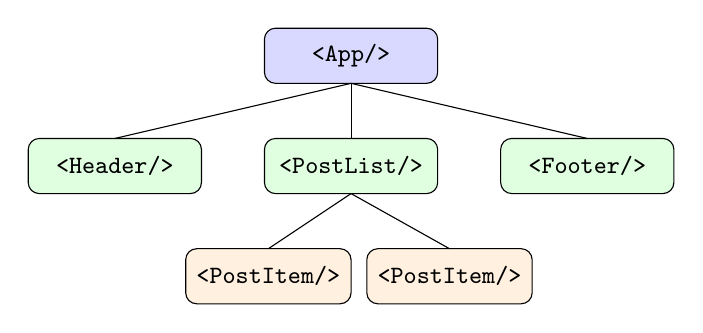
\begin{tikzpicture}[font=\small]
	\draw[fill=blue!15, rounded corners] (4.0,3.2) rectangle (6.2,3.9) node[midway]{\texttt{<App/>}};
	\draw[fill=green!12, rounded corners] (1.0,1.8) rectangle (3.2,2.5) node[midway]{\texttt{<Header/>}};
	\draw[fill=green!12, rounded corners] (4.0,1.8) rectangle (6.2,2.5) node[midway]{\texttt{<PostList/>}};
	\draw[fill=green!12, rounded corners] (7.0,1.8) rectangle (9.2,2.5) node[midway]{\texttt{<Footer/>}};
	\draw[fill=orange!12, rounded corners] (3.0,0.4) rectangle (5.1,1.1) node[midway]{\texttt{<PostItem/>}};
	\draw[fill=orange!12, rounded corners] (5.3,0.4) rectangle (7.4,1.1) node[midway]{\texttt{<PostItem/>}};
	\draw (5.1,3.2) -- (2.1,2.5); \draw (5.1,3.2) -- (5.1,2.5); \draw (5.1,3.2) -- (8.1,2.5);
	\draw (5.1,1.8) -- (4.05,1.1); \draw (5.1,1.8) -- (6.35,1.1);
\end{tikzpicture}
\end{center}
\vspace{0.5cm}
\noindent\textit{Figure~: arbre de composants — une UI React est une hiérarchie de composants réutilisables.}

\noindent \textbf{Règles de création} (AAV \og{}Appliquer les règles de création des composants\fg{})~: nom en \textbf{PascalCase} (\texttt{PostItem}), \textbf{responsabilité unique}, fonction \textbf{pure} (mêmes props → même rendu), \textbf{props en lecture seule} (jamais modifiées), retour d'un \textbf{seul élément racine}, et conception \textbf{réutilisable et indépendante}.

\newpage

\subsubsection*{React}
\phantomsection
\addcontentsline{toc}{subsection}{React}

\noindent \textbf{React} est une \textbf{bibliothèque JavaScript} front-end (créée par Facebook/Meta) servant à construire des interfaces utilisateur à base de \textbf{composants}. C'est le \textbf{framework Frontend} retenu pour le projet (AAV \og{}Utiliser un framework Frontend\fg{}). Ses principes fondateurs~:
\begin{itemize}
	\item \textbf{Déclaratif}~: on décrit l'interface en fonction de l'état~; React se charge de mettre à jour l'affichage.
	\item \textbf{Composants}~: l'UI est découpée en briques réutilisables.
	\item \textbf{Virtual DOM}~: React maintient une copie virtuelle du DOM et ne met à jour que ce qui change réellement, pour de bonnes \textbf{performances}.
	\item \textbf{Flux de données unidirectionnel}~: les données descendent du parent vers l'enfant via les props.
	\item \textbf{Hooks}~: fonctions (\texttt{useState}, \texttt{useEffect}…) qui ajoutent état et cycle de vie aux composants.
\end{itemize}

\subsubsection*{Front-end}
\phantomsection
\addcontentsline{toc}{subsection}{Front-end}

\noindent Le \textbf{front-end} désigne la \textbf{partie cliente} d'une application~: tout ce qui s'exécute dans le \textbf{navigateur} de l'utilisateur et avec quoi il interagit directement (l'interface, l'affichage, l'expérience utilisateur). Il est construit avec \textbf{HTML} (structure), \textbf{CSS} (style) et \textbf{JavaScript} (interactivité), ici via React et Tailwind. Il s'oppose au \textbf{back-end} (côté serveur~: logique métier, base de données, API) avec lequel il dialogue en échangeant du \textbf{JSON} via des requêtes HTTP.
\begin{center}
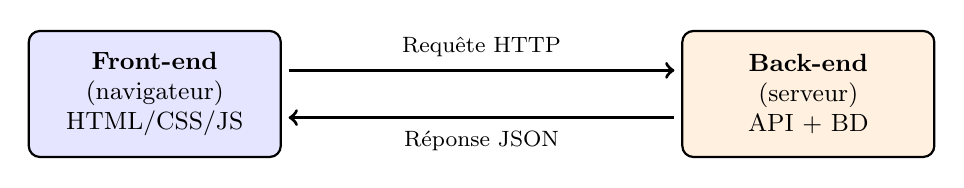
\begin{tikzpicture}[font=\small]
	\draw[thick, fill=blue!10, rounded corners] (0,0.4) rectangle (3.2,2) node[midway, align=center]{\textbf{Front-end}\\(navigateur)\\HTML/CSS/JS};
	\draw[thick, fill=orange!12, rounded corners] (8.3,0.4) rectangle (11.5,2) node[midway, align=center]{\textbf{Back-end}\\(serveur)\\API + BD};
	\draw[->, very thick] (3.3,1.5) -- (8.2,1.5); \node at (5.75,1.8) {\footnotesize Requête HTTP};
	\draw[<-, very thick] (3.3,0.9) -- (8.2,0.9); \node at (5.75,0.6) {\footnotesize Réponse JSON};
\end{tikzpicture}
\end{center}
\noindent\textit{Figure~: le front-end (client) dialogue avec le back-end (serveur) via HTTP/JSON.}

\subsubsection*{Wireframe}
\phantomsection
\addcontentsline{toc}{subsection}{Wireframe}

\noindent Un \textbf{wireframe} (\og{}maquette filaire\fg{}) est un \textbf{schéma simplifié, en basse fidélité}, de la structure d'une page ou d'un écran. Sans couleurs ni graphismes définitifs, il sert à positionner les \textbf{zones fonctionnelles} (en-tête, navigation, contenu, pied de page) et à valider l'\textbf{agencement} avant de coder. C'est un outil central de la \textbf{modélisation d'une application Frontend} (AAV) et un préalable au découpage en composants.
\vspace{0.2cm}
\begin{center}
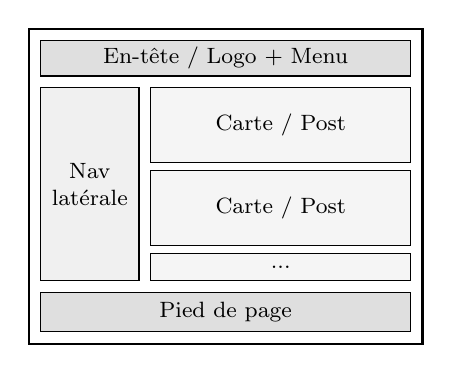
\begin{tikzpicture}[font=\footnotesize]
	\draw[thick] (0,0) rectangle (5,4);
	\draw[fill=gray!25] (0.15,3.4) rectangle (4.85,3.85) node[midway]{En-tête / Logo + Menu};
	\draw[fill=gray!12] (0.15,0.8) rectangle (1.4,3.25) node[midway, align=center]{Nav\\latérale};
	\draw[fill=gray!8] (1.55,2.3) rectangle (4.85,3.25) node[midway]{Carte / Post};
	\draw[fill=gray!8] (1.55,1.25) rectangle (4.85,2.2) node[midway]{Carte / Post};
	\draw[fill=gray!8] (1.55,0.8) rectangle (4.85,1.15) node[midway]{...};
	\draw[fill=gray!25] (0.15,0.15) rectangle (4.85,0.65) node[midway]{Pied de page};
\end{tikzpicture}
\end{center}
\noindent\textit{Figure~: wireframe d'une page — la structure est définie avant le style et le code.}

\subsubsection*{Redux}
\phantomsection
\addcontentsline{toc}{subsection}{Redux}

\noindent \textbf{Redux} est une bibliothèque de \textbf{gestion d'état global} pour les applications JavaScript (souvent associée à React). Quand un état doit être \textbf{partagé entre de nombreux composants} éloignés (utilisateur connecté, panier, liste de posts), le faire \og{}remonter\fg{} via les props devient ingérable. Redux centralise cet état dans un \textbf{store unique} et impose un \textbf{flux de données unidirectionnel et prévisible}~:
\begin{itemize}
	\item \textbf{Store}~: source de vérité unique contenant tout l'état.
	\item \textbf{Action}~: objet décrivant \og{}ce qui s'est passé\fg{} (ex.~: \texttt{\{ type: 'ADD\_POST' \}}).
	\item \textbf{Reducer}~: fonction pure qui calcule le \textbf{nouvel état} à partir de l'état courant et de l'action.
	\item \textbf{Dispatch}~: déclenche une action depuis l'interface.
\end{itemize}
\vspace{0.5cm}
\begin{center}
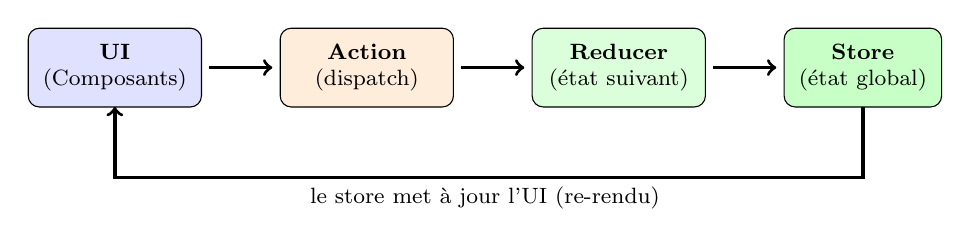
\begin{tikzpicture}[font=\footnotesize]
	\draw[fill=blue!12, rounded corners] (0,1.4) rectangle (2.2,2.4) node[midway, align=center]{\textbf{UI}\\(Composants)};
	\draw[fill=orange!14, rounded corners] (3.2,1.4) rectangle (5.4,2.4) node[midway, align=center]{\textbf{Action}\\(dispatch)};
	\draw[fill=green!14, rounded corners] (6.4,1.4) rectangle (8.6,2.4) node[midway, align=center]{\textbf{Reducer}\\(état suivant)};
	\draw[fill=green!22, rounded corners] (9.6,1.4) rectangle (11.6,2.4) node[midway, align=center]{\textbf{Store}\\(état global)};
	\draw[->, very thick] (2.3,1.9) -- (3.1,1.9);
	\draw[->, very thick] (5.5,1.9) -- (6.3,1.9);
	\draw[->, very thick] (8.7,1.9) -- (9.5,1.9);
	\draw[->, very thick] (10.6,1.4) -- (10.6,0.5) -- (1.1,0.5) -- (1.1,1.4);
	\node at (5.8,0.25) {\footnotesize le store met à jour l'UI (re-rendu)};
\end{tikzpicture}
\end{center}
\noindent\textit{Figure~: flux unidirectionnel de Redux — UI → action → reducer → store → UI.}

\subsubsection*{Tailwind CSS}
\phantomsection
\addcontentsline{toc}{subsection}{Tailwind CSS}

\noindent \textbf{Tailwind CSS} est un framework CSS dit \textbf{\og{}utility-first\fg{}}~: au lieu de fournir des composants pré-stylés (comme Bootstrap), il offre une multitude de \textbf{classes utilitaires} atomiques que l'on compose directement dans le HTML/JSX pour styliser élément par élément. Exemple~:
\begin{center}
\texttt{<button class="bg-blue-600 text-white px-4 py-2 rounded">Envoyer</button>}
\end{center}
\noindent Ici \texttt{bg-blue-600} (fond bleu), \texttt{text-white} (texte blanc), \texttt{px-4 py-2} (marges internes), \texttt{rounded} (coins arrondis). \textbf{Avantages}~: rapidité, cohérence visuelle, design \textbf{responsive} simple (\texttt{md:}, \texttt{lg:}), pas de feuilles CSS séparées à maintenir. C'est la \textbf{librairie de style} retenue (AAV \og{}Utiliser l'une des librairies de style\fg{}). \textbf{Différence avec Bootstrap}~: Bootstrap impose des composants tout faits (look reconnaissable), Tailwind laisse une liberté totale de design.

\newpage

\subsubsection*{useEffect}
\phantomsection
\addcontentsline{toc}{subsection}{useEffect}

\noindent \texttt{useEffect} est le \textbf{hook} React qui permet d'exécuter des \textbf{effets de bord} (actions extérieures au rendu)~: appels à une API, abonnements, minuteurs, manipulation directe du DOM. Il est \textbf{central pour gérer le cycle de vie} d'un composant (AAV \og{}Reconnaître les cycles de vie d'un composant\fg{}) et répond directement à la \textbf{problématique du projet} (chargement asynchrone des données). Son comportement dépend du \textbf{tableau de dépendances}~:
\begin{itemize}
	\item \texttt{useEffect(fn, [])}~: s'exécute \textbf{une seule fois au montage} — idéal pour charger les données initiales.
	\item \texttt{useEffect(fn, [x])}~: se ré-exécute à chaque changement de \texttt{x} (mise à jour).
	\item \textbf{Fonction de nettoyage} (\textit{return})~: exécutée au démontage, pour annuler abonnements/requêtes et éviter les fuites.
\end{itemize}
\vspace{0.5cm}
\begin{center}
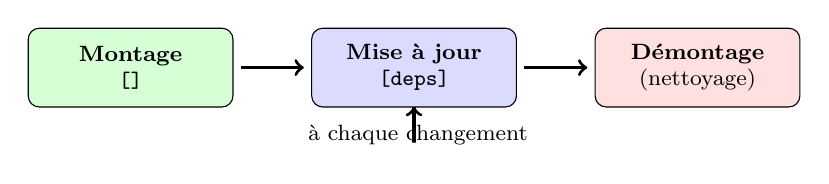
\begin{tikzpicture}[font=\footnotesize]
	\draw[fill=green!16, rounded corners] (0,0.8) rectangle (2.6,1.8) node[midway, align=center]{\textbf{Montage}\\\texttt{[]}};
	\draw[fill=blue!14, rounded corners] (3.6,0.8) rectangle (6.2,1.8) node[midway, align=center]{\textbf{Mise à jour}\\\texttt{[deps]}};
	\draw[fill=red!12, rounded corners] (7.2,0.8) rectangle (9.8,1.8) node[midway, align=center]{\textbf{Démontage}\\(nettoyage)};
	\draw[->, very thick] (2.7,1.3) -- (3.5,1.3);
	\draw[->, very thick] (6.3,1.3) -- (7.1,1.3);
	\draw[->, very thick] (4.9,0.8) .. controls (4.9,0.2) and (4.9,0.2) .. (4.9,0.8);
	\node at (4.9,0.45) {\footnotesize $\circlearrowright$ à chaque changement};
\end{tikzpicture}
\end{center}
\noindent\textit{Figure~: les trois phases du cycle de vie pilotées par \texttt{useEffect}.} Dans le projet, on charge les données dans un \texttt{useEffect([])} et on affiche un état de chargement tant que le JSON n'est pas arrivé — ce qui élimine les erreurs d'initialisation décrites dans le contexte.

\subsubsection*{Axios}
\phantomsection
\addcontentsline{toc}{subsection}{Axios}

\noindent \textbf{Axios} est une bibliothèque cliente \textbf{HTTP basée sur les promesses} (\textit{Promise}) permettant au front-end d'effectuer des \textbf{requêtes asynchrones} vers une API REST (GET, POST, PUT, DELETE) et d'en récupérer les données. Atouts par rapport au \texttt{fetch} natif~: conversion \textbf{automatique en JSON}, gestion simplifiée des erreurs, en-têtes et intercepteurs, délais d'attente. Couplé à \texttt{useEffect}, il constitue le mécanisme de \textbf{chargement asynchrone} des données~:
\vspace{0.5cm}
\begin{center}
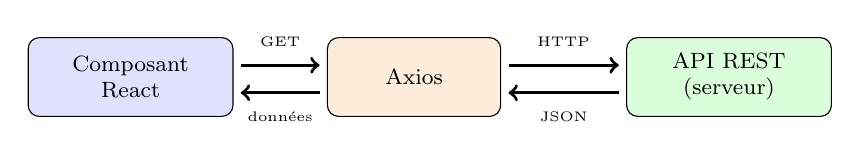
\begin{tikzpicture}[font=\footnotesize]
	\draw[fill=blue!12, rounded corners] (0,0.6) rectangle (2.6,1.6) node[midway, align=center]{Composant\\React};
	\draw[fill=orange!14, rounded corners] (3.8,0.6) rectangle (6.0,1.6) node[midway]{Axios};
	\draw[fill=green!14, rounded corners] (7.6,0.6) rectangle (10.2,1.6) node[midway, align=center]{API REST\\(serveur)};
	\draw[->, very thick] (2.7,1.25) -- (3.7,1.25); \node at (3.2,1.55){\tiny GET};
	\draw[->, very thick] (6.1,1.25) -- (7.5,1.25); \node at (6.8,1.55){\tiny HTTP};
	\draw[<-, very thick] (6.1,0.9) -- (7.5,0.9); \node at (6.8,0.6){\tiny JSON};
	\draw[<-, very thick] (2.7,0.9) -- (3.7,0.9); \node at (3.2,0.6){\tiny données};
\end{tikzpicture}
\end{center}
\noindent\textit{Figure~: Axios fait le pont asynchrone entre le composant React et l'API REST.}

\newpage

\subsubsection*{DOM}
\phantomsection
\addcontentsline{toc}{subsection}{DOM}

\noindent Le \textbf{DOM} (\textit{Document Object Model}) est la \textbf{représentation en mémoire, sous forme d'arbre}, de la page HTML telle qu'interprétée par le navigateur. Chaque balise HTML y devient un \textbf{n\oe ud} manipulable par JavaScript (créer, modifier, supprimer des éléments, réagir aux événements). C'est via le DOM que l'interface est réellement affichée et mise à jour.
\vspace{0.5cm}
\begin{center}
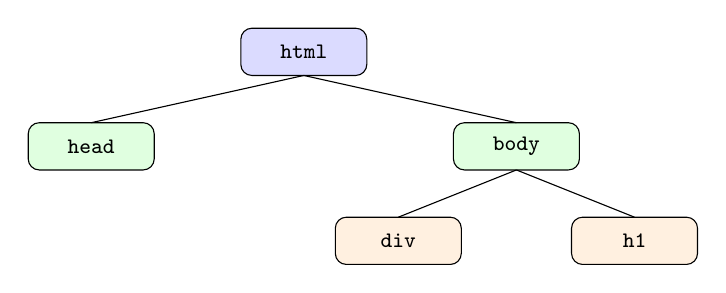
\begin{tikzpicture}[font=\footnotesize]
	\draw[fill=blue!14, rounded corners] (4.2,3.2) rectangle (5.8,3.8) node[midway]{\texttt{html}};
	\draw[fill=green!12, rounded corners] (1.5,2.0) rectangle (3.1,2.6) node[midway]{\texttt{head}};
	\draw[fill=green!12, rounded corners] (6.9,2.0) rectangle (8.5,2.6) node[midway]{\texttt{body}};
	\draw[fill=orange!12, rounded corners] (5.4,0.8) rectangle (7.0,1.4) node[midway]{\texttt{div}};
	\draw[fill=orange!12, rounded corners] (8.4,0.8) rectangle (10.0,1.4) node[midway]{\texttt{h1}};
	\draw (5.0,3.2) -- (2.3,2.6); \draw (5.0,3.2) -- (7.7,2.6);
	\draw (7.7,2.0) -- (6.2,1.4); \draw (7.7,2.0) -- (9.2,1.4);
\end{tikzpicture}
\end{center}
\vspace{0.5cm}

\noindent\textit{Figure~: le DOM, arbre des n\oe uds de la page.} React n'agit pas directement sur ce DOM réel (coûteux)~: il passe par un \textbf{Virtual DOM}, en calcule les différences, et ne met à jour que les n\oe uds modifiés — d'où ses bonnes \textbf{performances}.

\newpage

\section*{Analyse et résolution : Front-end}
\addcontentsline{toc}{section}{Analyse et résolution : Front-end}

\noindent \textit{Rappel de la problématique~:} \og{}Comment gérer efficacement le cycle de vie des composants et le chargement asynchrone des données dans une application React pour éviter les erreurs d'affichage~?\fg{}

\vspace{0.3cm}

\noindent Pour y répondre, nous traitons successivement les quatre facettes du problème~: \textbf{(1)} la \textbf{modélisation} de l'interface et son découpage en composants, \textbf{(2)} le \textbf{cycle de vie} d'un composant et le hook \texttt{useEffect}, \textbf{(3)} le \textbf{chargement asynchrone} des données (Axios) et la \textbf{gestion des états} qui élimine les erreurs d'affichage, \textbf{(4)} l'\textbf{état global} (Redux) et le \textbf{style} (Tailwind). Une synthèse argumentée clôt l'analyse.

\vspace{0.4cm}

\subsection*{1. Modélisation et découpage en composants}
\phantomsection
\addcontentsline{toc}{subsection}{1. Modélisation et découpage en composants}
\noindent La conception débute \textbf{avant le code} par un \textbf{wireframe} qui fixe la structure des écrans (en-tête, navigation, contenu, pied de page). Ce découpage se traduit ensuite en un \textbf{arbre de composants} où chaque zone fonctionnelle devient une brique autonome (\texttt{<Header/>}, \texttt{<PostList/>}, \texttt{<PostItem/>}, \texttt{<Footer/>}). Les \textbf{règles de création} sont appliquées~: nom en \textbf{PascalCase}, \textbf{responsabilité unique}, fonction \textbf{pure}, \textbf{props en lecture seule} et \textbf{réutilisabilité}. Un composant feuille typique ne fait que recevoir des props et retourner du JSX~:

\begin{minted}[fontsize=\footnotesize, bgcolor=gray!8]{jsx}
// PostItem.jsx -- composant pur, réutilisable, props en lecture seule
function PostItem({ auteur, contenu }) {
  return (
    <li className="p-4 rounded shadow bg-white">
      <strong>{auteur}</strong> : {contenu}
    </li>
  );
}
\end{minted}

\vspace{0.3cm}

\subsection*{2. Cycle de vie et hook \texttt{useEffect}}
\phantomsection
\addcontentsline{toc}{subsection}{2. Cycle de vie et useEffect}
\noindent Un composant traverse trois phases~: le \textbf{montage} (première insertion dans le DOM), les \textbf{mises à jour} (re-rendus déclenchés par un changement d'état ou de props) et le \textbf{démontage} (retrait du DOM). L'erreur décrite dans le contexte vient d'un \textbf{mauvais placement de la logique de chargement}~: si l'on tente d'exploiter les données pendant le rendu, le composant s'exécute \textbf{avant} l'arrivée du JSON. La solution consiste à déporter l'appel réseau dans un \texttt{useEffect} déclenché \textbf{au montage} (tableau de dépendances vide \texttt{[]})~: le rendu n'attend pas le réseau, et c'est l'arrivée des données qui provoque un re-rendu propre.

\newpage

\subsection*{3. Chargement asynchrone et gestion des états}
\phantomsection
\addcontentsline{toc}{subsection}{3. Chargement asynchrone et gestion des états}
\noindent Le c\oe ur de la résolution combine \textbf{Axios} (requête HTTP asynchrone, JSON déjà parsé) avec \textbf{trois états} maintenus par \texttt{useState}~: les \textbf{données}, un indicateur de \textbf{chargement} et une éventuelle \textbf{erreur}. L'appel est lancé au montage et une \textbf{fonction de nettoyage} annule la requête au démontage (\texttt{AbortController}), évitant les fuites et les mises à jour sur composant démonté.

\begin{minted}[fontsize=\footnotesize, bgcolor=gray!8]{jsx}
import { useState, useEffect } from 'react';
import axios from 'axios';

function PostList() {
  const [posts, setPosts]       = useState([]);    // données (JSON -> objets)
  const [chargement, setLoad]   = useState(true);  // état de chargement
  const [erreur, setErreur]     = useState(null);  // état d'erreur

  useEffect(() => {
    const controleur = new AbortController();       // annulation au démontage

    axios.get('/api/posts', { signal: controleur.signal })
      .then((reponse) => setPosts(reponse.data))    // JSON déjà parsé par Axios
      .catch((err) => { if (!axios.isCancel(err)) setErreur(err); })
      .finally(() => setLoad(false));

    return () => controleur.abort();                // nettoyage (démontage)
  }, []);                                           // [] -> une fois, au montage
\end{minted}

\noindent Le \textbf{rendu conditionnel} garantit ensuite que l'on n'affiche \textbf{jamais} la liste tant que les données ne sont pas disponibles~: c'est précisément ce qui \textbf{supprime les erreurs d'affichage} de la problématique.

\begin{minted}[fontsize=\footnotesize, bgcolor=gray!8]{jsx}
  if (chargement) return <p className="text-gray-500">Chargement...</p>;
  if (erreur)     return <p className="text-red-600">Erreur de chargement.</p>;

  return (
    <ul className="space-y-2">
      {posts.map((post) => (
        <PostItem key={post.id} auteur={post.auteur} contenu={post.contenu} />
      ))}
    </ul>
  );
}
\end{minted}

\noindent Tant que \texttt{chargement} est vrai, l'interface affiche un indicateur~; en cas d'échec, un message d'erreur~; ce n'est qu'\textbf{une fois le JSON arrivé} que la liste est rendue. Le composant est ainsi \textbf{robuste à l'asynchronisme}, ce qui répond directement au contexte (rendu déclenché avant la disponibilité des données).

\newpage

\subsection*{4. État global (Redux) et style (Tailwind)}
\phantomsection
\addcontentsline{toc}{subsection}{4. État global et style}
\noindent Lorsqu'une donnée doit être \textbf{partagée entre de nombreux composants éloignés} (utilisateur connecté, liste de posts mutualisée), la faire transiter par les props devient ingérable. \textbf{Redux} centralise alors cet état dans un \textbf{store unique} au flux unidirectionnel et prévisible (\textit{action} → \textit{reducer} → \textit{store} → re-rendu de l'UI), ce qui rend l'évolution de l'application plus lisible et testable.

\vspace{0.2cm}

\noindent Côté présentation, \textbf{Tailwind CSS} (\textit{utility-first}) applique le style directement dans le JSX via des classes atomiques (\texttt{p-4}, \texttt{rounded}, \texttt{bg-white}, \texttt{text-red-600}…), comme dans les extraits ci-dessus. On obtient un rendu \textbf{cohérent et responsive} sans feuille CSS séparée à maintenir.

\vspace{0.4cm}

\subsection*{Synthèse}
\phantomsection
\addcontentsline{toc}{subsection}{Synthèse}
\noindent La réponse à la problématique tient en une chaîne cohérente~: \textbf{modéliser} (wireframe → arbre de composants), \textbf{isoler l'asynchrone} dans un \texttt{useEffect} de montage, \textbf{charger} via Axios en pilotant trois états (données / chargement / erreur), \textbf{rendre conditionnellement} pour ne jamais afficher de données absentes, et \textbf{nettoyer} au démontage. Redux et Tailwind complètent la pile pour l'état partagé et le style. Cette démarche élimine les erreurs d'initialisation et constitue un \textbf{patron reproductible} pour toute page consommant une API.

\newpage

\subsection*{Conclusion}
\phantomsection
\addcontentsline{toc}{subsection}{Conclusion}

\noindent \textbf{En réponse à la problématique}, l'analyse a montré que gérer efficacement le cycle de vie des composants et le chargement asynchrone des données ne relève pas d'une astuce isolée, mais d'une \textbf{chaîne de décisions cohérentes}. Tout part de la \textbf{modélisation}~: un wireframe fixe la structure des écrans, traduite en un \textbf{arbre de composants} modulaires, purs et réutilisables (PascalCase, responsabilité unique, props en lecture seule).

\vspace{0.2cm}

\noindent Le c\oe ur de la résolution est le \textbf{placement correct de la logique asynchrone}~: l'appel réseau est déporté dans un \texttt{useEffect} déclenché au \textbf{montage} (\texttt{[]}), de sorte que le rendu n'attend jamais le réseau. \textbf{Axios} récupère le \textbf{JSON} et alimente trois états (\texttt{données}, \texttt{chargement}, \texttt{erreur}) qui pilotent un \textbf{rendu conditionnel}~: on n'affiche la liste qu'une fois les données présentes. C'est ce mécanisme qui \textbf{supprime les erreurs d'affichage} décrites dans le contexte. Une \textbf{fonction de nettoyage} (\texttt{AbortController}) annule la requête au démontage et évite les fuites mémoire.

\vspace{0.2cm}

\noindent Pour l'état partagé entre composants éloignés, \textbf{Redux} centralise les données dans un store unique au flux unidirectionnel et prévisible, tandis que \textbf{Tailwind CSS} assure un style cohérent et responsive directement dans le JSX. Au final, la pile \textbf{React + Axios + Redux + Tailwind} satisfait l'ensemble des AAV visés et constitue un \textbf{patron reproductible} pour le développement front-end des futures applications de l'entreprise.

\newpage

\section*{Capitalisation}
\addcontentsline{toc}{section}{Capitalisation}

\begin{center}
\setlength{\tabcolsep}{10pt}

\begin{tabular}{|p{0.30\textwidth}|p{0.45\textwidth}|m{0.08\textwidth}|}
\hline
\textbf{AAV} & \textbf{Commentaire} & \textbf{Statut} \\ \hline

Appliquer les règles de création des composants &
Règles détaillées (PascalCase, responsabilité unique, fonction pure, props en lecture seule, racine unique) et mises en \oe uvre dans le composant \texttt{PostItem} de l'analyse. &
{\color{green!60!black}Acquis} \\ \hline

Construire et manipuler des données en JSON &
Structure du JSON (objets/tableaux) expliquée~; réponse d'API récupérée via Axios (\texttt{reponse.data}) puis parcourue (\texttt{.map}) pour alimenter les composants. &
{\color{green!60!black}Acquis} \\ \hline

Reconnaître les cycles de vie d'un composant &
Phases montage / mise à jour / démontage schématisées et pilotées par \texttt{useEffect} (dépendances \texttt{[]}, nettoyage par \texttt{AbortController}) dans le code de résolution. &
{\color{green!60!black}Acquis} \\ \hline

Réaliser la modélisation d'une application Frontend &
Modélisation par wireframes (structure des écrans) puis découpage en arbre de composants, repris comme point de départ de l'analyse. &
{\color{green!60!black}Acquis} \\ \hline

Utiliser un framework Frontend &
React expliqué (composants, déclaratif, Virtual DOM, flux unidirectionnel, hooks) et appliqué concrètement (\texttt{useState}/\texttt{useEffect}, rendu conditionnel) pour résoudre la problématique. &
{\color{green!60!black}Acquis} \\ \hline

Utiliser l'une des librairies de style (Bootstrap, Tailwind, etc.) &
Tailwind CSS (utility-first) présenté avec exemple de classes, comparé à Bootstrap et utilisé directement dans le JSX des extraits de l'analyse. &
{\color{green!60!black}Acquis} \\ \hline

\end{tabular}
\end{center}

\newpage

\section*{Ressources}
\addcontentsline{toc}{section}{Ressources}

\begin{itemize}
	\item \textbf{Documentation React} : \url{https://react.dev/}
	\item \textbf{Hook useEffect (cycle de vie)} : \url{https://react.dev/reference/react/useEffect}
	\item \textbf{Documentation Tailwind CSS} : \url{https://tailwindcss.com/docs}
	\item \textbf{Documentation Redux / Redux Toolkit} : \url{https://redux.js.org/}
	\item \textbf{Documentation Axios} : \url{https://axios-http.com/fr/docs/intro}
	\item \textbf{JSON (MDN)} : \url{https://developer.mozilla.org/fr/docs/Web/JavaScript/Reference/Global_Objects/JSON}
	\item \textbf{DOM (MDN)} : \url{https://developer.mozilla.org/fr/docs/Web/API/Document_Object_Model}
	\item \textbf{Next.js (framework React)} : \url{https://nextjs.org/docs}
\end{itemize}
